\subsection{Understanding Impedance: The Mystery of a Shorted 1/2-Wavelength Line!}

\begin{tcolorbox}[colback=gray!10, colframe=black, title=E9F04] What impedance does a 1/2-wavelength transmission line present to an RF generator when the line is shorted at the far end?
\begin{enumerate}[label=\Alph*.]
    \item Very high impedance
    \item \textbf{Very low impedance}
    \item The same as the characteristic impedance of the line
    \item The same as the output impedance of the RF generator
\end{enumerate} \end{tcolorbox}

\subsubsection{Related Concepts}

To understand this question, we need to delve into the concepts of transmission lines, impedance, reflection, and RF (Radio Frequency) systems. When we discuss a transmission line, we refer to a specialized cable or structure designed to carry RF signals from one location to another. 

\textbf{1. Impedance::} This is the measure of how much resistance an electrical circuit presents to the flow of alternating current (AC) at a given frequency. The characteristic impedance (\(Z_0\)) of a transmission line is a key parameter and is defined as:
\[
Z_0 = \sqrt{\frac{L}{C}}
\]
where \(L\) is the inductance per unit length and \(C\) is the capacitance per unit length of the line.

\textbf{2. 1/2-Wavelength Transmission Line::} A 1/2-wavelength transmission line is one that has a length equal to half the wavelength (\(\lambda/2\)) of the signal it is carrying. This specific length has unique properties concerning impedance and voltage standing wave ratio (VSWR).

\textbf{3. Short Circuit at the Far End::} When the line is shorted at its far end (i.e., the impedance at the end of the transmission line is 0 ohms), it significantly affects how the line behaves.

\textbf{Reflection of Waves::} When a signal travels down a transmission line and encounters a discontinuity (like a short circuit), part of the signal is reflected back. The impedance that is seen at the input of the transmission line depends on the load at the far end.

\textbf{Calculation of Input Impedance::} For a shorted transmission line of length \(L = \frac{\lambda}{2}\), the input impedance (\(Z_{in}\)) can be determined by the formula:
\[
Z_{in} = j Z_0 \tan(\beta L)
\]
where:
- \(j\) is the imaginary unit,
- \(\beta\) is the phase constant, which for a 1/2-wavelength line becomes \(\pi\),
- \(Z_0\) is the characteristic impedance of the transmission line.

Substituting \(L = \frac{\lambda}{2}\):
\[
Z_{in} = j Z_0 \tan\left(\pi\right) = jZ_0 \times 0 = 0
\]

Thus, the input impedance at the RF generator is very low, confirming that the correct answer to the question is (B) Very low impedance.

\subsubsection{Visual Representation}

To provide a better understanding, we can visualize the transmission line and the short circuit using a simple TikZ diagram:

\begin{center}
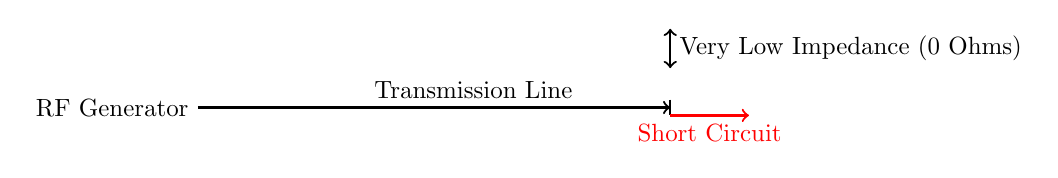
\begin{tikzpicture}[thick, scale=1.0, every node/.style={scale=0.9}]

    % Drawing the transmission line
    \draw[->] (0,0) -- (5,0) node[midway, above] {Transmission Line};
    
    % Short circuit at the far end
    \draw[thick] (5,0.1) -- (5,-0.1);
    \draw[->, red] (5,-0.1) -- (6,-0.1) node[midway, below] {Short Circuit};
    
    % Drawing RF generator
    \draw[thick] (-1,0) node[left] {RF Generator} -- (0,0);
    
    % Indicating the impedance
    \draw[<->] (5,0.5) -- (5,1) node[midway, right] {Very Low Impedance (0 Ohms)};

\end{tikzpicture}
\end{center}
